\newchapstyle
\chapter{Introduction}
\label{chap:intro}

%\epigraph[0pt]{
%    Failure is not an option.
%}{Actor Ed Harris, playing flight director Gene Kranz, in the 1995 film Apollo 13\cite{FailureNotOption2019}}

%\begin{abstract}
%Lorem ipsum dolor sit amet, consectetur adipisicing elit, sed do eiusmod tempor incididunt ut labore et dolore magna aliqua. Ut enim ad minim veniam, quis nostrud exercitation ullamco laboris nisi ut aliquip ex ea commodo consequat. Duis aute irure dolor in reprehenderit in voluptate velit esse cillum dolore eu fugiat nulla pariatur. Excepteur sint occaecat cupidatat non proident, sunt in culpa qui officia deserunt mollit anim id est laborum.
%\end{abstract}

%% Start the actual chapter on a new page.
\afterpage{\pagecolor{none}}\newpage

\section{Computing with semi- and superconducting circuits}

The information age and the underlying development of the metal oxide semiconductor field-effect transistor (MOSFET, cf. Fig.~\ref{fig:introcomputing}(a)) lay the ground to the world which we know today.
%
Pushed by continuous advances in material sciences, solid state physics and electrical engineering, the MOSFET is now the building block of all commercial computers.
%
Owed largely by the success of scalability from integrated circuits, state-of-the-art microprocessors host more than 39.54 billion transistors on a single chip, with physical dimensions down to a few tens of nanometers, cf. Fig.~\ref{fig:introcomputing}(b)~\cite{mujtabaAMDEPYCRome2019}.
%
With the increasing transistor density and shrinking physical dimensions came however the realization, that alternative computation architectures to the one based on semiconducting transistors might be needed to satisfy society's desire for information, as there might be a limit to how dense logic circuits might be packed with current technology as the number of transistors on a chip were found to double every two years~\cite{mooreCrammingMoreComponents2006}.

Based on Feynman's ideas of building quantum machines to run the most complex calculations much more efficient than any digital one, MOSFET-based, computer could, the late twentieth century saw the birth of first prototypes based on a quantum computing architecture~\cite{feynmanSimulatingPhysicsComputers1982}.
%
Since then, the buzz on "quantum computing" is all around us, with global tech companies like IBM~\cite{steffenQuantumComputingIBM2011}, Google~\cite{aruteQuantumSupremacyUsing2019}, Microsoft~\cite{linnNewMicrosoftBreakthroughs2020} and Intel~\cite{vandersypenQuantumComputingSemiconductor2019} all heavily invested and following slightly different paths.
%
One promising approach relies on Josephson junctions, which are weak links between two superconducting banks, as the building block for a superconducting quantum computing architecture.
%
While, superconducting circuits were already envisioned in the first half of the twentieth century as a competitive alternative to semiconducting computers~\cite{brockWillNSAFinally}, Josephson junctions spured additional interest due to their sensitive nature to magnetic flux and potentially much higher switching speeds compared to MOSFETs~\cite{josephsonPossibleNewEffects1962,andersonProbableObservationJosephson1963}.
%
In parallel to the development of MOSFETs, Josephson junctions were hence envisioned as building blocks for superconducting logic circuits, with IBM being one of the main drivers at the time~\cite{anackerJosephsonComputerTechnology1980a}.
%
In an attempt to combine the best of two worlds, the versatility of a high gain transistor, and the low dissipation of superconducting circuits, proposals were made in the 1980s to merge these two elements into the Josephson field effect transistor (JoFET), cf. Fig.~\ref{fig:introcomputing}(c)~\cite{clarkFeasibilityHybridJosephson1980,gallagherThreeterminalSuperconductingDevices1985}.
%
Yet, IBM eventually seized to research Josephson junction computation due to an apparent supremacy of semiconducting computers~\cite{robinsonIBMDropsSuperconducting1983}.

Research continued however at public institutions and universities, and soon it was realized that Josephson junctions could form the basis of quantum bits~\cite{martinisQuantumJosephsonJunction2020}.
%
Since then, superconducting quantum processors based on Josephson junctions embedded in microwave circuits, as pursued by IBM and Google, have culminated in the milestone "quantum supremacy", i.e. the threshold at which a quantum processor became capable of executing an algorithm that would be prohibitively costly in terms of computing time and money for a classical computer to perform~\cite{aruteQuantumSupremacyUsing2019}.
%
The building block of these processors are superconducting quantum interference devices (SQUIDs, cf. Fig.~\ref{fig:introcomputing}(e,f)) formed by two Josephson junctions in a loop.

To tune the states of these qubits, magnetic flux is threaded through the SQUID loop, supplied via on-chip current bias lines in close proximity of the SQUIDs.
%
However, these magnetic fields come with a few drawbacks:
%
Already the very first implementation of such a two-qubit processor showed that these magnetic fields can lead to significant cross talk coupling qubits several centimeters apart from each other\cite{dicarloDemonstrationTwoqubitAlgorithms2009}.
%
Additionally, the dilution refrigerators cooling the chips to isolate them from thermal fluctuations only have limited cooling power which can be exceeded if enough current is put on chip.
%
As the number of physical qubits increases, so does the challenge of shielding individual qubits from each other's bias lines, and retaining enough cooling power as to not induce thermal effects.

In comparison, replacing SQUIDs with the long-abandoned JoFET might be beneficial:
%
Applying gate voltages instead of running a current through a wire is non-dissipative, which removes the cooling power constraint.
%
Additionally, cross-talk would be significantly reduced due to the nature of electric fields in gate capacitors being strongly confined to a small volume around the gate voltage lead.
%
Finally, JoFETs have consistently performed well under application of in-plane magnetic fields.
%
While the latter are not strictly necessary in transmon qubits, flux noise is one of the limiting factors of SQUIDs.
%
Even more important, magnetic fields are one of the requirements of qubits based on the Majorana architecture~\cite{hyartFluxcontrolledQuantumComputation2013}, which rules out aluminum oxide junctions and necessitates JoFETs.


As of now, there has been only very little research in integrating JoFETs in superconducting qubits.
%
Most notably, semiconductor nanowires and epitaxial 2DEGs were integrated in transmon qubits, resulting in so-called "gatemons", cf. Fig.~\ref{fig:introcomputing}(d)~\cite{delangeRealizationMicrowaveQuantum2015,larsenSemiconductorNanowireBasedSuperconductingQubit2015,casparisGatemonBenchmarkingTwoQubit2016a,casparisSuperconductingGatemonQubit2018,luthiEvolutionNanowireTransmon2018}.
%
While coherence times are not yet at the same level as for standard transmons, gatemons show great promise and have gained significant interest in the scientific community.
%
Gatemons not only provide a new way of qubit control~\cite{shimSemiconductorinspiredDesignPrinciples2016}, but also a path towards studying unconventional superconducting weak links at high frequencies~\cite{tahanGrapheneQubitMotivates2019}.


\begin{figure}[t]
	\centering
	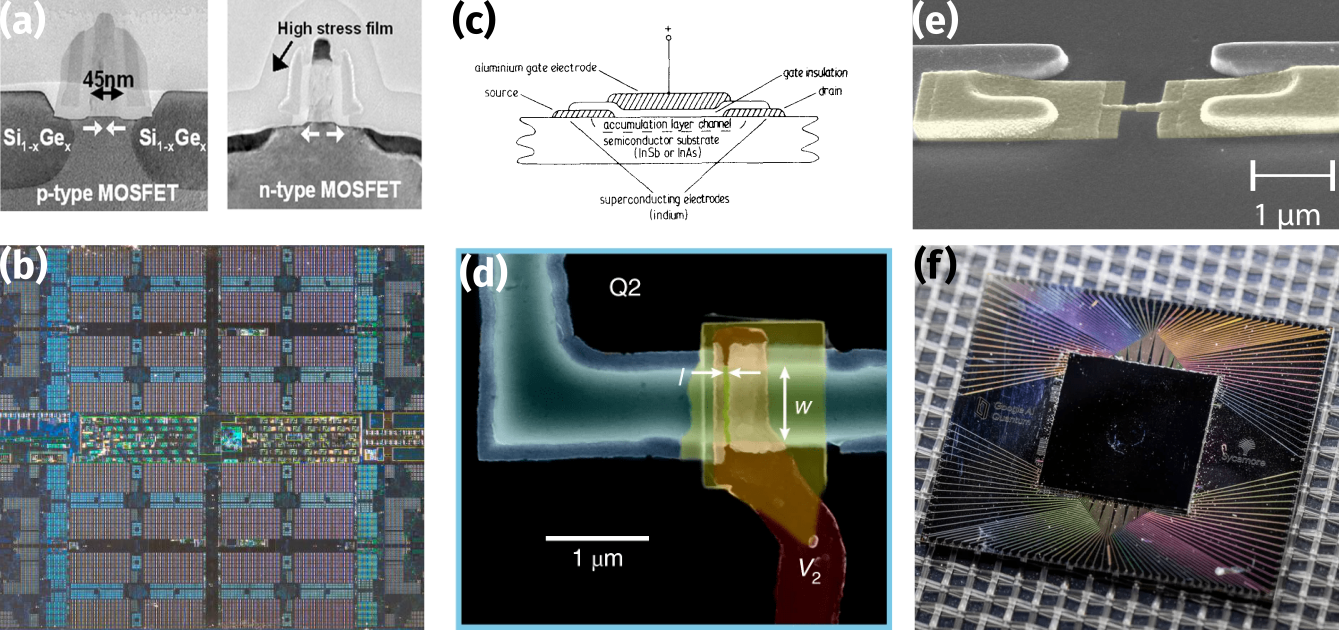
\includegraphics[width=\linewidth]{chapter-introduction/figs/intro_computing.svg.png}
	\caption{
		\textbf{Semi- and superconducting based computing devices.}
		%
		\textbf{(a)} Cross-sectional TEM image of \SI{45}{\nano\meter} node MOSFETs, the building block of semiconducting computers, adapted from~\cite{thompsonLogicNanotechnologyFeaturing2004}.
		%
		\textbf{(b)} Die shot of part of the I/O die of the microprocessor with currently highest number of transistors, in this case with \SI{14}{\nano\meter} node: The \textit{AMD Epyc Rome} with \num{8.34e9} transistors on the I/D die and \num{39.54e9} total, adapted from \cite{mujtabaAMDEPYCRome2019}.
		%
		\textbf{(c)} Sketch of the first envisioned JoFET as hybrid between semiconducting transistors and superconducting Josephson junctions, adapted from~\cite{clarkFeasibilityHybridJosephson1980}.
		%
		\textbf{(d)} SEM of a single-qubit gatemon, a potential computation basis for a hybrid super-semi approach, adapted from~\cite{casparisSuperconductingGatemonQubit2018}.
		%
		\textbf{(e)} SEM of an aluminum oxide Josephson junction, the workhorse of the superconducting quantum computing architecture, adapted from~\cite{langfordExperimentallySimulatingDynamics2017}.
		%
		\textbf{(f)} Optical image of Google's "quantum supremacy" 53 qubit \textit{Sycamore} quantum processor, adapted from~\cite{shanklandTakeLookGoogle2020}. 
	}
	\label{fig:introcomputing}
\end{figure}


In this thesis, we initially set out to explore how graphene Josephson junctions could perform in superconducting microwave circuits.
%
Since its discovery in 2004, graphene has shown versatile field effect applications and, already since very early on, gate-tunable superconductivity~\cite{novoselovElectricFieldEffect2004c,heerscheBipolarSupercurrentGraphene2007a}.
%
With improvements on contact engineering and reduced film disorder, induced superconductivity in graphene Josephson has been a testbed for Andreev physics, phase coherence, quantum phase transitions and the interplay of superconductivity and magnetism ~\cite{leeProximityCouplingSuperconductorgraphene2018a}.
%
Incorporating these devices in microwave circuits thus is a first step towards the realization of gate-tunable superconducting microwave logic circuits.
%
However, to not lose the information about the device's DC properties, and to directly link them to the microwave performance, we chose to combine both DC and MW in one device, by utilizing DC bias cavities~\cite{bosmanBroadbandArchitectureGalvanically2015c}.
%
This not only allows for a detailed study of the junction's properties, but also enables applications based on current-biasing the device.







\section{Josephson effects in SNS systems}

\begin{figure}[t]
	\centering
	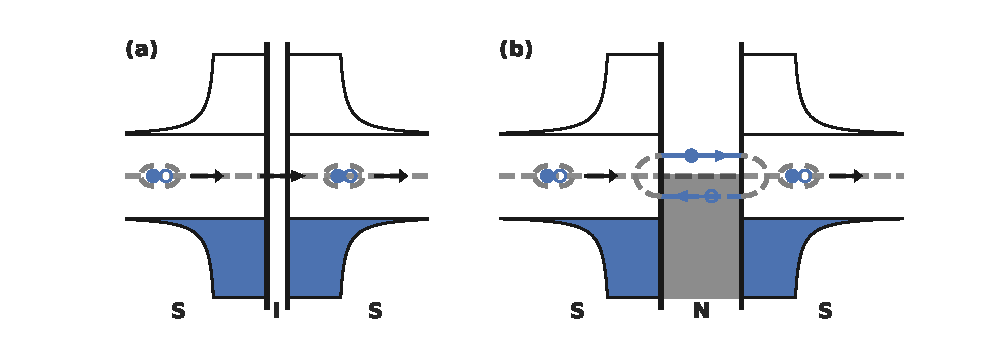
\includegraphics[width=\linewidth]{chapter-introduction/figs/model_SNS_DOS}
	\caption{
		\textbf{Cooper pair transport in SIS and SNS Josephson junctions.}
		%
		The density of states in a superconductor exhibits a gap of width $2\Delta$ in energy around the Fermi level $\epsilon_F$, with states below $\epsilon_F$ filled and states above unoccupied.
		%
		\textbf{(a)} In an SIS Josephson junction, Cooper pairs, consisting of an electron and hole with opposite spins can tunnel through a thin insulating barrier separating two superconducting banks.
		%
		There are no states inside the insulating region.
		%
		\textbf{(b)} In an SNS Josephson junction, the normal region exhibits a DOS that is filled up to $\epsilon_F$.
		%
		Cooper pairs entering the normal region are broken up into electrons and holes of opposite spin and momentum, that can enter the superconductor under Andreev reflection, thus forming Andreev bound states within the normal region.
		%
		This results in a net current across the junction.
	}
	\label{fig:modelsnsdos}
\end{figure}

Josephson junctions have been used widely in the field of superconducting circuits.
%
Already their first applications were thought of as the building block for superconducting logical circuits.

The process of Andreev reflection at the interface between superconductors and normal metals lays the fundament for understanding how a Josephson junction works.
%
The process is sketched in Fig. \ref{fig:modelsnsdos}:
%
An electron impinging onto the super-normal interface from inside the normal region can only enter the superconductor in the form of a Cooper pair by being reflected as a hole with opposite spin and momentum.
%
Vice versa, a Cooper pair travelling towards the normal region will decay into an electron travelling forward, and annihilate a hole travelling backwards with spin opposite to that of the electron.
%
Inside the normal region, this will result in the formation of the so-called Andreev bound states (ABS).

Since inside the superconductor, there are no states allowed for $\epsilon_F - \Delta \leq \epsilon_F \leq \epsilon_F - \Delta$, the superconducting electrodes can be though of as forming potential barriers at the interface, leading to transparencies $\tau$, and the Andreev paris can be thought of analogously as particles inside a box.
%
\textbf{TODO!!! ?? Here also elaborate on the Thouless energy and 2D junctions.}


Nanda \textit{et al.}~\cite{nandaCurrentPhaseRelationBallistic2017} point out an important factor to take into account:
%
Skewness can quite significantly depend on the S-N interface, i.e. transparency, and the ratio $L/\xi$.
%
Temperature additionally suppresses skewness, since this leads to a higher number of quasiparticles, and increases the amount of continuum states contributing to the supercurrent.

Let us consider a 1-dimensional SNS junction with perfect contact transparency $\tau_c=1$ at the SN interface.
%
Then each Andreev bound state has a ground state energy
%
\begin{align}
E_{i}^{\rm ABS} = -\Delta\sqrt{1-T_i\sin^2(\delta/2)}
\end{align}
%
with induced superconducting gap $\Delta$ and channel transparency $T_i$, where $T_i$ takes into account scattering inside the normal region.
%
The energy of the excited ABS has opposite sign.
%
Summing over all of these channels, the total Josephson potential is given by
%
\begin{align}
U_J(\delta) = 1-\sum_i E_{i}^{\rm ABS} \approx E_J \frac{\delta^2}{2} - E_J\left( 1-\frac{3\sum T_i^2}{4\sum T_i} \right) \frac{\delta^4}{24} +\mathcal{O}(\delta^6)%\ , \\
%E_J &= \frac{\Delta}{4}\sum_i T_i \rightarrow \frac{\Delta}{4}N\tau
\end{align}
%
In the limit of low $T_i$, i.e. for an SIS junction, the energy would be given simply by $U_J^{\rm SIS}(\delta)=1-\Delta\cos(\delta)\approx E_J\delta^2/2-E_J\delta^4/24$.
%
Compared to the SIS case, the Josephson energy is reduced by a fraction depending on the channel transparency which will become important later on.
%
We plot the ground and excited state energies of the ABS in Fig.~\ref{fig:modelsnsejic}(a).
%
With increasing channel transmission, $U_J$ exhibits stronger modulation and a closing band gap at $\delta=\pi$ with minimum separation $2\Delta\sqrt{1-\tau}$.

\begin{figure}[t]
	\centering
	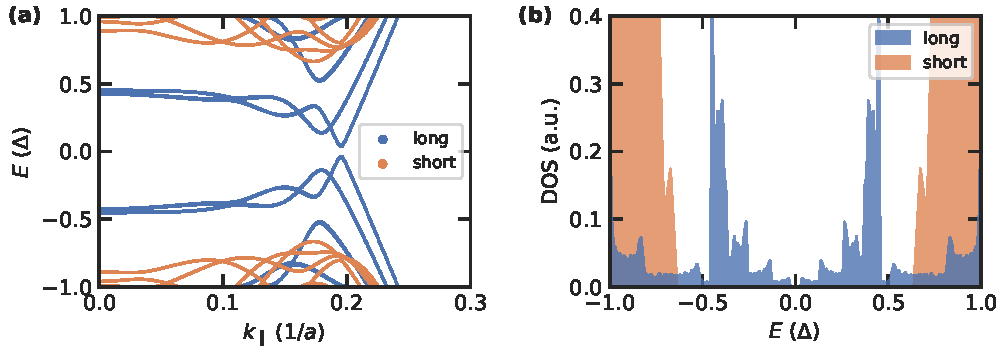
\includegraphics[width=\linewidth]{chapter-introduction/figs/kwant_modeling_181206_subgap_length_supp_Plot_subgap_dos}
	\caption{
		\textbf{Realistic subgap states of a 2D graphene Josephson junction.}
		%
		Tight-binding simulations of a graphene Josephson junction show strong dependence of the subgap state energies on momentum parallel to the SN interface \textbf{(a)}, with lowest lying energies at large $k_\parallel$.
		%
		While the short JJ (orange) shows an only slightly reduced minimum energy and DOS \textbf{(b)} compared to $\Delta$, long junctions (blue) exhibit heavily reduced energy gaps.
	}
	\label{fig:modelsubgap}
\end{figure}

The exact nature of the subgap states however depends on a multitude of parameters, such as the crystal structure, size and geometry of the junction, as well as the contact transparency.
%
Figure~\ref{fig:modelsubgap} shows the calculated subgap density of states for a basic graphene Josephson junction and the influence of these parameters.
%
Most notably in comparison to the basic ABS energy, contact transparency $\tau_c<1$ leads to the ABS detaching from the bulk gap at $\Delta$ even for zero phase difference~\cite{bretheauTunnellingSpectroscopyAndreev2017a}.
%
Additionally, the longer the junction, i.e. the further the superconducting banks are spaced apart, the lower the resulting ABS energy, since the superconducting phase decays exponentially in the normal conductor.
%
In the case of a 2D junction, large junction width, i.e. lateral extensions, additionally reduce the ABS energy.




Turning back to the basic 1D-ABS picture, the corresponding Josephson current and inductance are 
\begin{align}
I(\delta) &= \frac{2e}{\hbar}\frac{\partial U_J}{\partial\delta} = \frac{e\Delta}{2\hbar}\sum_i\frac{T_i\sin\delta}{\sqrt{1-T_i\sin^2\delta/2}} \\
L_J(\delta) &= \frac{\hbar}{2e}\left( \frac{\partial I_J}{\partial\delta} \right)^{-1} = \left(\frac{\hbar}{2e}\right)^2\left(\frac{\partial^2U_J}{\partial\delta^2}\right)^{-1} \\
&= \frac{4\hbar^2}{e^2\Delta}\sum_i \frac{\left(1-T_i\sin^2(\delta/2)\right)^{3/2}}{4T_i\cos\delta\left(1-T_i\sin^2(\delta/2)\right)+T_i^2\sin^2(\delta)}
\end{align}

Both quantities are depicted in Fig.~\ref{fig:modelsnsejic}.
%
We can conclude two things:
%
First, the larger the channel transmission, the stronger the forward skew of the current phase relation and corresponding deviation to the SIS case.
%
Second, while also strongly nonlinear, the Josephson inductance of SNS junctions is significantly reduced compared to the SIS case.

In order to build reliable, reproducible circuits out of SNS junctions, it is thus vital to characterize them not only in the DC, but also in the microwave regime, as this is where the inductance will be measurable.
%
To this end, we placed our junctions in a circuit allowing for steady and high frequency signals to probe our device.
%
These DC bias microwave circuits are described in the following section.

\begin{figure}[t]
	\centering
	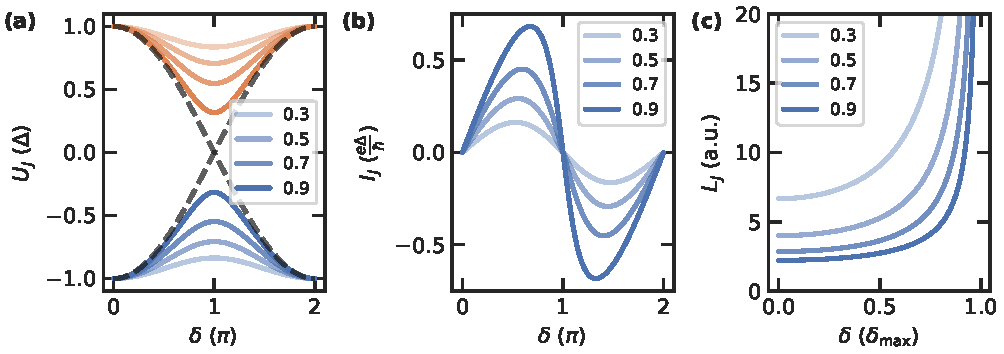
\includegraphics[width=\linewidth]{chapter-introduction/figs/model_SNS_EjIc}
	\caption{
		\textbf{Channel transmission and nonsinusoidality.}
		%
		\textbf{(a)} Josephson energy of the ground (blue) and excited (orange) Andreev bound state for varying channel transmission $\tau$ as a function of phase drop across the Josephson junction.
		%
		Increasing color intensity corresponds to increasing $\tau$.
		%
		Finite contact transparency $\tau_c<1$ at the SN interface detaches the ABS energy from the bulk gap $\pm\Delta$ (dashed line).
		%
		\textbf{(b)} Josephson current for varying $\tau$.
		%
		Increasing transmission increases both amplitude and forward skewing of the CPR.
		%
		\textbf{(c)} Josephson inductance as a function of phase normalized to the one at maximum $L_J$.
		%
		Due to the increased CPR slope for increasing $\tau$ at zero phase, the Josephson inductance decreases significantly.
	}
	\label{fig:modelsnsejic}
\end{figure}


\section{DC bias cavities for probing Josephson junctions}

\begin{figure}[t]
	\centering
	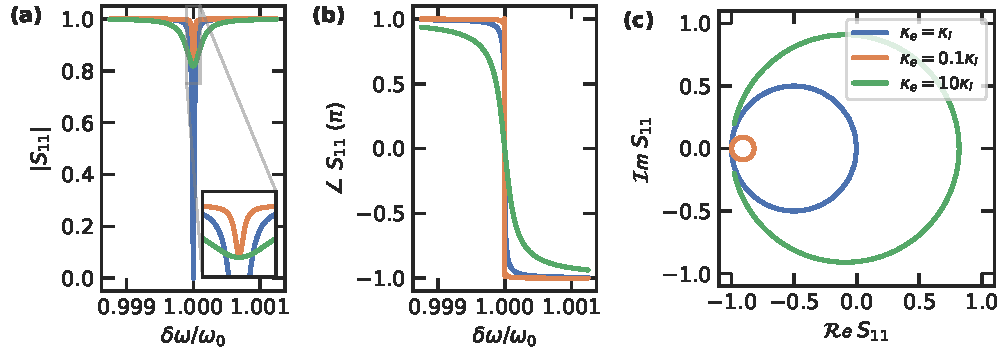
\includegraphics[width=\linewidth]{chapter-introduction/figs/model_DC_bias_cavity_coupling.pdf}
	\caption{
		\textbf{Effect of coupling ratio of the reflection coefficient of a DC bias cavity.}
		%
		Using Eq.~\ref{eq:intro-s11}, we can model the absolute value \textbf{(a)}, phase \textbf{(b)} and real and imaginary parts \textbf{(c)} of the reflection coefficient of a DC bias cavity.
		%
		Colors denote the various coupling types: blue: critically coupled $\kappa_e/\kappa_i=1$, orange: undercoupled $\kappa_e/\kappa_i=0.1$, green: overcoupled $\kappa_e/\kappa_i=10$.
		%
		Best signal-to-noise ratio is achieved for critical coupling, while the other two cases have identical SNR in terms of $\abs{S_{11}}$.
	}
	\label{fig:s11}
\end{figure}


In order to probe the Josephson inductance, we make use of superconducting microwave resonators based on coplanar waveguides~\cite{gopplCoplanarWaveguideResonators2008,zmuidzinasSuperconductingMicroresonatorsPhysics2012}.
%
These have been used extensively in the field of particle detection and circuit (quantum) electrodynamics due to the intrinsic low loss originating from the absence in resistance of the Cooper pairs~\cite{dayBroadbandSuperconductingDetector2003a,blaisCavityQuantumElectrodynamics2004c,clerkHybridQuantumSystems2020,blaisQuantumInformationProcessing2020}.
%
In order to analyze our devices both in the low and high frequency range (DC to several $\SI{e9}{\hertz}$), our circuits need to be able to sustain relatively large quality factors while being able to introduce direct current and voltage access to the device under test (DUT).

While there is a variety of circuit architectures capable of this approach, such as using inductive coupling~\cite{vissersFrequencytunableSuperconductingResonators2015b}, direct leads at voltage nodes of a $\lambda/2$ resonator with matching length~\cite{chenIntroductionDcBias2011a,liApplyingDirectCurrent2013} or lumped-element split-cavities~\cite{mahashabdeFastTunableHigh2020}, we based our design on an architecture previously developed in our group, the shunt capacitor DC bias access~\cite{bosmanBroadbandArchitectureGalvanically2015c}.
%
The advantage of this approach is threefold:
%
As no circuit symmetries need to be considered, the design is rather simple.
%
No additional port needs to be used to probe or excite the DUT, thus there is no additional leakage channel.
%
Finally, using a shunt capacitor provides a broadband signal port up to the self-resonance of the shunt capacitor, which is chosen to be well above the resonance frequency of the circuit.

Figure~\ref{fig:TLmodel}(a) depicts a schematic of the DC bias cavity circuit.
%
In principle, measurements in both transmission and reflection geometry are possible.
%
However, we typically use the second port for supplying a DC gate voltage, and short the DUT to ground.
%
Therefore, we only perform reflection measurements.

The reflection coefficient of this circuit is given by
%
\begin{align}
S_{11}=-1+\frac{2\kappa_e}{\kappa_e+\kappa_i+2i\Delta}
\label{eq:intro-s11}
\end{align}
%
with the internal and external loss rates $\kappa_i$ and $\kappa_e$ and the detuning $\Delta=\omega-\omega_0$~\cite{bosmanBroadbandArchitectureGalvanically2015c}.
%
In Fig.~\ref{fig:s11} we plot the reflection coefficient for various fractions of $\eta =\kappa_e/\kappa_i$, to illustrate the effects of over-, under- and critical coupling ($\eta >1$, $\eta <1$ and $\eta =1$, respectively).
%
For a best signal-to-noise ratio, the shunt capacitor $C_s$ should be designed such that $\kappa_e=\kappa_i$, with the external loss rate approximately given by
%
\begin{align}
\kappa_e &= \frac{\omega_0}{Q_e} = \frac{2}{\pi\omega_0Z_0^2C_s^2}
\label{eq:intro-kappae}
\end{align}
%
with external quality factor $Q_e$ and transmission line impedance $Z_0$.
%
However, when placing a JJ at the end of the TL, the internal loss rate can rise significantly.
%
For this reason, we typically design our circuits such that they are overcoupled without a JJ present, anticipating a rise in $\kappa_i$.
%
As shown in the inset of Fig.~\ref{fig:s11}(a), over- or undercoupling by the same factor in fact leads to the same SNR in the absolute value of $S_{11}$.
%
It is tempting to therefore search for a circuit resonance in the measured since this provides a potentially more reliable identification method.
%
Nevertheless, measurement background from impedance mismatches, resulting in oscillations of the background, often obscure even drastic phase changes, for which reason the absolute value can at times be better suited.

\begin{figure}
	\centering
	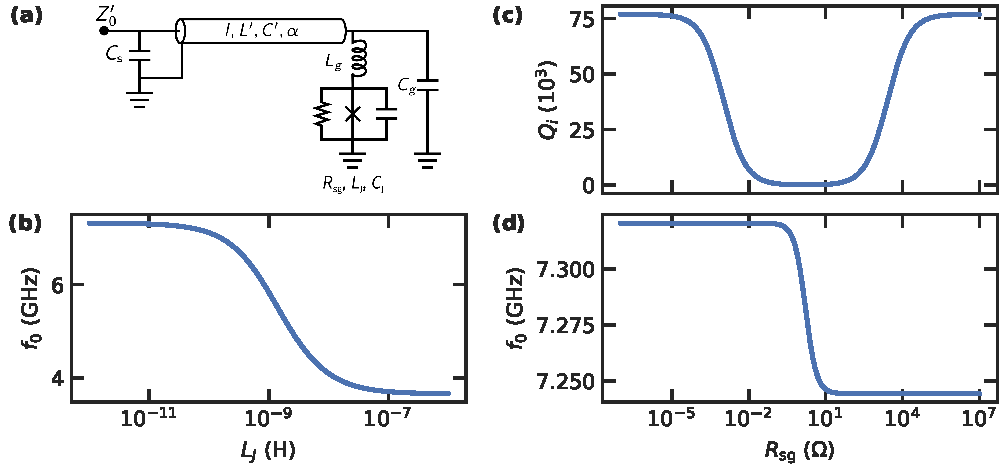
\includegraphics[width=\linewidth]{chapter-introduction/figs/model_DC_bias_cavity_params_RCSJ.pdf}
	\caption{
		\textbf{DC bias cavity shorted to ground by a parametrized top-gated graphene Josephson junction.}
		%
		\textbf{(a)} Fully parametrized circuit model.
		%
		The transmission line is described by length $l$, inductance and capacitance per unit length $L^\prime$ and $C^\prime$ and attenuation $\alpha$, and is coupled to an input impedance $z_0^\prime$ via a shunt capacitance $C_s$.
		%
		The Josephson junction is modeled as a network of linear lead inductance $L_g$ together with an RCSJ model of subgap-resistance $R_{\rm sg}$, junction capacitance $C_J$, nonlinear inductance $L_J$ and gate capacitance $C_g$.
		%
		\textbf{(b)} Resonance frequency versus Josephson inductance with the other parameters fixed.
		%
		Depending on the junction impedance, the fundamental cavity mode changes from $\lambda/2$ (small $L_J$) to $\lambda/4$ (large $L_J$).
		%
		\textbf{(c,d)} Influence on subgap resistance on internal quality factor and resonance frequency.
		%
		Very small $R_{\rm sg}$ corresponds to a short, very large $R_{\rm sg}$ to an open to ground in parallel with $L_J$.
		%
		In both cases, the internal losses are dominated by the transmission line attenuation.
		%
		For intermediate values of $R_{\rm sg}$, significant resistive damping effectively suppresses the circuit response.
		%
		Panel \textbf{(d)} also illustrates the shift of $f_0$ due to $L_J$ as in panel \textbf{(b)} when changing the boundary condition.
	}
	\label{fig:TLmodel}
\end{figure}


When probing Josephson junctions with the DC bias cavity, we need to calibrate the microwave circuit parameters.
%
This is done by measuring a combination of an open and shorted reference device with the same sample geometry, except with an open or short to ground in place of the JJ.
%
Equipped with these values, we can proceed to extract information about the JJ:
%
With an added Josephson junction with inductance $L_J$ shorting the TL to ground, the shifted resonance frequency can be approximated by
%
\begin{align}
\omega_0^\prime = \omega_0\frac{L_r+L_J}{L_r+2L_J}
\label{eq:intro-omega0p}
\end{align}
%
where $L_r$ is the lumped TL resonator inductance including geometric and kinetic inductances, cf. Chapter~\ref{chap:gJJ-CPR} and Fig.~\ref{fig:TLmodel}(b).
%
A complete analytical model of an RSCJ model parametrizing the JJ can be used for calculating junction-induced losses in the form of a subgap resistance, cf. Chapter~\ref{chap:gJJ} and Fig.~\ref{fig:TLmodel}.
%
For very small $R_{\rm sg}$, the Josephson inductance is effectively short-circuited, so $Q_i$ approaches the limit of no JJ.
%
On the other hand, very large $R_{\rm sg}$ implies an open circuit with no losses other than the ones in the TL resonator, again approaching $Q_i$ of the bare cavity.
%
Intermediate resistance values suppress the resonance entirely.
%
The shift in $f_0$ for large $R_{\rm sg}$ shows the frequency shift induced by $L_J$.



\section{Outline}

In the following, we will show the applications of DC bias cavities to both extract information about the intrinsic parameters of the Josephson junctions to be probed, and use the combination of cavity and junction to perform a detection measurement.


In chapter~\ref{chap:experiment}, we provide a detailed overview on the experimental methods that we developed and used to enable the measurements presented later on.
%
We detail the exfoliation and fabrication of van der Waals devices, superconducting CPW resonators.
%
Additionally, a short introduction to the use of the superconducting alloy molybdenum-rhenium in Delft, together with a small study on its pros and cons, is supplied.
%
This chapter also includes a brief introduction to thermal noise and the fridge wiring used to suppress the former during measurements.

In chapter~\ref{chap:gJJ}, we present the first measurements of a graphene Josephson junction in the microwave regime.
%
Motivated by the potential use of graphene in superconducting quantum circuits, we studied the Josephson inductance by tracking the resonance frequency, and high-frequency losses of the junction attributed to its subgap resistance by extracting the added circuit losses.
%
Together with a detailed circuit characterization in both DC and the MW regime, the results indicate that graphene Josephson junctions are indeed a feasible platform for circuit quantum electrodynamics.


In chapter~\ref{chap:gJJ-CPR}, we take a closer look at the underlying mechanisms governing the Josephson inductance of graphene Josephson junctions, i.e. their current-phase relation.
%
Using previously not performed microwave measurements of DC bias cavities, we show that the CPR of diffusive and ballistic devices is forward-skewed, as is expected for these junctions.
%
We quantify the resulting correction of the Josephson energy potential, which is crucial for the use of gJJs in microwave quantum circuits.

We end the part of this thesis concerned with graphene devices with chapter~\ref{chap:gJJ-misc}.
%
Here, we provide a collection of additional DC data on graphene Josephson junctions and SQUIDs.
%
In particular, we investigate oscillations in the IV curves that occur as a result of the junction probing its electromagnetic environment in the absence, and the phase locking to the presence of microwave radiation, resulting in Fiske and Shapiro steps, respectively.


We switch from pure fundamental studies of the junction's characteristics to a circuit application in chapter~\ref{chap:currentdetection}.
%
Instead of a graphene JoFET, we present a DC bias MW cavity coupled to an aluminum constriction Josephson junction, a so-called Dayem bridge~\cite{andersonRadioFrequencyEffectsSuperconducting1964}.
%
Making use of the responsivity of the circuit's resonance frequency to bias current, we detect low-frequency currents with a minimum measured sensitivity of \SI{8.9}{\pico\ampere\per\hertz\tothe{1/2}}, comparable to state-of-the-art devices.
%
With an analytical circuit model, we extrapolate orders of magnitude better values for improved device designs based on our circuit, which could eventually enable quantum limited current detection.


We close with a summary of all presented results and a possible way onwards in chapter~\ref{chap:conclusion}.
%
Additional information on tips and tricks for electron beam lithography, such as alignment and height measurements, useful source code and specifications on the self-assembled low-pass and copper powder filters are appended to this thesis.


%\clearpage
%\references{dissertation}

